% Options for packages loaded elsewhere
\PassOptionsToPackage{unicode}{hyperref}
\PassOptionsToPackage{hyphens}{url}
\PassOptionsToPackage{dvipsnames,svgnames,x11names}{xcolor}
%
\documentclass[
  letterpaper,
  DIV=11,
  numbers=noendperiod]{scrartcl}

\usepackage{amsmath,amssymb}
\usepackage{iftex}
\ifPDFTeX
  \usepackage[T1]{fontenc}
  \usepackage[utf8]{inputenc}
  \usepackage{textcomp} % provide euro and other symbols
\else % if luatex or xetex
  \usepackage{unicode-math}
  \defaultfontfeatures{Scale=MatchLowercase}
  \defaultfontfeatures[\rmfamily]{Ligatures=TeX,Scale=1}
\fi
\usepackage{lmodern}
\ifPDFTeX\else  
    % xetex/luatex font selection
\fi
% Use upquote if available, for straight quotes in verbatim environments
\IfFileExists{upquote.sty}{\usepackage{upquote}}{}
\IfFileExists{microtype.sty}{% use microtype if available
  \usepackage[]{microtype}
  \UseMicrotypeSet[protrusion]{basicmath} % disable protrusion for tt fonts
}{}
\makeatletter
\@ifundefined{KOMAClassName}{% if non-KOMA class
  \IfFileExists{parskip.sty}{%
    \usepackage{parskip}
  }{% else
    \setlength{\parindent}{0pt}
    \setlength{\parskip}{6pt plus 2pt minus 1pt}}
}{% if KOMA class
  \KOMAoptions{parskip=half}}
\makeatother
\usepackage{xcolor}
\setlength{\emergencystretch}{3em} % prevent overfull lines
\setcounter{secnumdepth}{-\maxdimen} % remove section numbering
% Make \paragraph and \subparagraph free-standing
\makeatletter
\ifx\paragraph\undefined\else
  \let\oldparagraph\paragraph
  \renewcommand{\paragraph}{
    \@ifstar
      \xxxParagraphStar
      \xxxParagraphNoStar
  }
  \newcommand{\xxxParagraphStar}[1]{\oldparagraph*{#1}\mbox{}}
  \newcommand{\xxxParagraphNoStar}[1]{\oldparagraph{#1}\mbox{}}
\fi
\ifx\subparagraph\undefined\else
  \let\oldsubparagraph\subparagraph
  \renewcommand{\subparagraph}{
    \@ifstar
      \xxxSubParagraphStar
      \xxxSubParagraphNoStar
  }
  \newcommand{\xxxSubParagraphStar}[1]{\oldsubparagraph*{#1}\mbox{}}
  \newcommand{\xxxSubParagraphNoStar}[1]{\oldsubparagraph{#1}\mbox{}}
\fi
\makeatother


\providecommand{\tightlist}{%
  \setlength{\itemsep}{0pt}\setlength{\parskip}{0pt}}\usepackage{longtable,booktabs,array}
\usepackage{calc} % for calculating minipage widths
% Correct order of tables after \paragraph or \subparagraph
\usepackage{etoolbox}
\makeatletter
\patchcmd\longtable{\par}{\if@noskipsec\mbox{}\fi\par}{}{}
\makeatother
% Allow footnotes in longtable head/foot
\IfFileExists{footnotehyper.sty}{\usepackage{footnotehyper}}{\usepackage{footnote}}
\makesavenoteenv{longtable}
\usepackage{graphicx}
\makeatletter
\def\maxwidth{\ifdim\Gin@nat@width>\linewidth\linewidth\else\Gin@nat@width\fi}
\def\maxheight{\ifdim\Gin@nat@height>\textheight\textheight\else\Gin@nat@height\fi}
\makeatother
% Scale images if necessary, so that they will not overflow the page
% margins by default, and it is still possible to overwrite the defaults
% using explicit options in \includegraphics[width, height, ...]{}
\setkeys{Gin}{width=\maxwidth,height=\maxheight,keepaspectratio}
% Set default figure placement to htbp
\makeatletter
\def\fps@figure{htbp}
\makeatother

\KOMAoption{captions}{tableheading}
\makeatletter
\@ifpackageloaded{caption}{}{\usepackage{caption}}
\AtBeginDocument{%
\ifdefined\contentsname
  \renewcommand*\contentsname{Table of contents}
\else
  \newcommand\contentsname{Table of contents}
\fi
\ifdefined\listfigurename
  \renewcommand*\listfigurename{List of Figures}
\else
  \newcommand\listfigurename{List of Figures}
\fi
\ifdefined\listtablename
  \renewcommand*\listtablename{List of Tables}
\else
  \newcommand\listtablename{List of Tables}
\fi
\ifdefined\figurename
  \renewcommand*\figurename{Figure}
\else
  \newcommand\figurename{Figure}
\fi
\ifdefined\tablename
  \renewcommand*\tablename{Table}
\else
  \newcommand\tablename{Table}
\fi
}
\@ifpackageloaded{float}{}{\usepackage{float}}
\floatstyle{ruled}
\@ifundefined{c@chapter}{\newfloat{codelisting}{h}{lop}}{\newfloat{codelisting}{h}{lop}[chapter]}
\floatname{codelisting}{Listing}
\newcommand*\listoflistings{\listof{codelisting}{List of Listings}}
\makeatother
\makeatletter
\makeatother
\makeatletter
\@ifpackageloaded{caption}{}{\usepackage{caption}}
\@ifpackageloaded{subcaption}{}{\usepackage{subcaption}}
\makeatother
\ifLuaTeX
  \usepackage{selnolig}  % disable illegal ligatures
\fi
\usepackage[]{natbib}
\bibliographystyle{plainnat}
\usepackage{bookmark}

\IfFileExists{xurl.sty}{\usepackage{xurl}}{} % add URL line breaks if available
\urlstyle{same} % disable monospaced font for URLs
\hypersetup{
  pdftitle={On a Alvenicity of solar wind discontinuities},
  colorlinks=true,
  linkcolor={blue},
  filecolor={Maroon},
  citecolor={Blue},
  urlcolor={Blue},
  pdfcreator={LaTeX via pandoc}}

\title{On a Alvenicity of solar wind discontinuities}
\author{Zijin Zhang \and Sergei Kamaletdinov \and Xiaofei Shi \and Anton V. Artemyev \and Marco Velli \and Vassilis Angelopoulos}
\date{}

\begin{document}
\maketitle
\begin{abstract}
Solar wind plasma flow is characterized by intense, large-amplitude current sheets, also known as solar wind discontinuities. These regions are believed to play a crucial role in magnetic reconnection, solar wind ion heating, and energetic particle scattering. Although solar wind discontinuities share several properties with the classical MHD model of rotational discontinuities, they exhibit more complex characteristics that include many kinetic properties, going beyond this model. One of the most puzzling properties of these discontinuities is their Alvenicity, which describes the relationship between Alfvén and plasma velocity jumps across discontinuities. Although the high correlation of these jumps suggests the rotational nature of discontinuities, the significant differences in jump amplitudes indicate the necessity of kinetic mechanisms to describe the stress balance within discontinuities. Spacecraft observations show that plasma thermal anisotropy alone may not sufficiently explain this difference and achieve stress balance. In this study, we present a theoretical model in which this difference is explained by the kinetics of interpenetrating ion beams crossing the discontinuity. Our model successfully describes the observed properties of discontinuities within the inner heliosphere.
\end{abstract}

\newcommand{\vect}[1]{\mathbf{#1}}

\section{References}\label{references}

\begin{itemize}
\tightlist
\item
  \citet{steinhauerMultifluidModelOnedimensional2008}
\item
  \citet{artemyevIonNongyrotropySolar2020}
\item
  \citet{neukirchKineticModelsTangential2020}
\item
  \citet{vaskoThinCurrentSheets2014}
\end{itemize}

\section{Introduction}\label{introduction}

\begin{enumerate}
\def\labelenumi{\arabic{enumi}.}
\tightlist
\item
  Observation features of solar wind discontinuities
\item
  The necessity of kinetic models to describe solar wind discontinuities
\item
  Current theoretical models of solar wind discontinuities and their limitations
\end{enumerate}

\begin{itemize}
\tightlist
\item
  Harris current sheet \citet{harrisPlasmaSheathSeparating1962}
\end{itemize}

Observations of magnetic discontinuities exhibit Alfvenic properties, with the plasma velocity variation correlating well with magnetic field components variations. However, the amplitude of the plasma velocity jump is often significantly smaller than the Alfvén velocity jump, indicating a more complicated picture than the classical MHD model of rotational discontinuities. Figure~\ref{fig-examples} show observations of magnetic discontinuities in different regions of the heliosphere, PSP within 0.2 AU, Wind upstream of the Earth's bow shock, and ARTEMIS in the Earth's magnetotail. Previously, this discrepancy has been interpreted as a possible contribution of anisotropy that decreases the Alfvén velocity jump, or a discontinuity non-stationarity due to residual magnetic energy, or an ion nonadiabatic interaction with intense (thin) discontinuities that shapes the nongyrotropic ion distribution to include a nondiagonal term of the pressure tensor, with a cross-discontinuity gradient decreasing the Alfvén velocity jump \citet{artemyevIonNongyrotropySolar2020}.

These differences could not be simply explained by the aniostropy of the plasma thermal pressure alone (assuming a Maxwellian distribution that fits both the parallel and perpendicular temperatures) and suggest that kinetic mechanisms are necessary to describe the stress balance within discontinuities.

\begin{figure}

\centering{

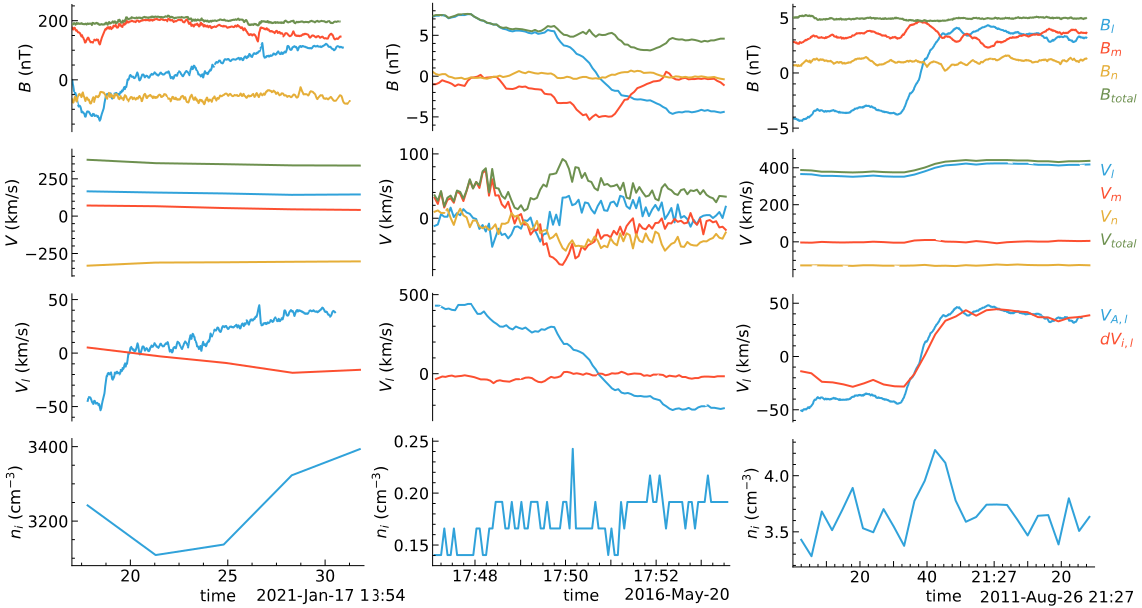
\includegraphics{article_files/mediabag/figures/fig_examples.pdf}

}

\caption{\label{fig-examples}Three examples of solar wind discontinuities observed by Parker Solar Probe (PSP), ARTEMIS and Wind spacecraft with sub-Alfvenic flow velocity.}

\end{figure}%

Force-free \citet{harrisonRemarksOnedimensionalForcefree2009} (A necessary condition on the pseudopotential plasma pressure to allow for force-free 1D VM equilibria is formulated.)

\section{Multifluid Model}\label{multifluid-model}

We used a steady-state multi-fluid model for assumed 1-D force-free current sheets. This approach, inspired by \citet{steinhauerMultifluidModelOnedimensional2008}, has the advantage of being analytically tractable while providing the necessary complexity to include the kinetic effects of multiple ion species. Kinetic approach, which is in principle more accurate, is hard to solve analytically and difficult to interpret the measurements. The multifluid model is a good compromise between the simplicity of the MHD model and the complexity of the kinetic model. One disadvantage of the multifluid model, however, is that there are more unknowns than equations. This means that the model is underdetermined and requires additional assumptions to be solved. This closure problem is usually solved by choosing equations of state. In this study, we first attempted to solve the system with a scalar pressure model, but then the system was overdetermined and no solution was found. We avoid this problem by assuming a specific profile for one of the variables, which is then used to solve the rest of the system.

\section{Plasma-Field Equations for Force-free current sheet}\label{plasma-field-equations-for-force-free-current-sheet}

Following \citet{steinhauerMultifluidModelOnedimensional2008}, we consider a one-dimensional force-free current sheet where \(B_x^2 + B_y^2 = B_0^2 = \text{const}\), with all variables dependent solely on \(z\). The system comprises multiple steady-state ion species (fluid groups) and a background electron fluid.

Electron motion is along the field lines \(\mathbf{u_e} = Γ_e \mathbf{B} / (n_e B_z)\). And the conservation of fluid mass \(d(n_α u_{αz})/dz = 0\) integrate to a constant parameters \(Γ_α = n_α u_{αz}\). The momentum equations for each ion species are given by

\begin{equation}\phantomsection\label{eq-momentum}{
\begin{aligned}
Γ_α \frac{d u_{α x}}{d z} &= n_α u_{α y} B_z - Γ_α B_y
\\
Γ_α \frac{d u_{α y}}{d z} &= Γ_α B_x-n_α u_{α x} B_z
\\
Γ_α \frac{d u_{α z}}{d z} &= -\frac{1}{2} \frac{d p_α}{d z}-n_α \frac{d \phi}{d z}+n_α u_{α x} B_y-n_α u_{α y} B_x
\end{aligned}
}\end{equation}

Ampere's law connects the fields and the flow components

\begin{equation}\phantomsection\label{eq-Jx}{
d B_y / d z = - J_x = - \sum_α n_α u_{α x} + n_e u_{e x} = -n u_x+\Gamma_e B_x / B_z
}\end{equation}

\begin{equation}\phantomsection\label{eq-Jy}{
d B_x / d z = J_y = \sum_α n_α u_{α y} - n_e u_{e y} = n u_y-\Gamma_e B_y / B_z
}\end{equation}

\begin{equation}\phantomsection\label{eq-Jz}{
d B_z / d z = J_z = \sum_α n_α u_{α z} - n_e u_{e z} = n u_z-\Gamma_e
}\end{equation}

And the Gauss's law for magnetism gives another constant parameter \(B_{z} = \text{const}\).

This is a system of \(3N+2\) equations for \(4N+2\) unknown dependent variables: \(B_x\), \(B_y\), and \(N\) each of \(n\), \(p\), \(u_x\), and \(u_y\). Since we are interested in force-free solutions with \(B_x^2 + B_y^2 = B_0^2 = \text{const}\), this condition provides an additional equation for the system.

A scalar pressure model, which provides another N equations connecting \(p\) and \(n\), was attempted as per \citet{steinhauerMultifluidModelOnedimensional2008}, but no solution was found (the system was overdetermined). Therefore, the system is considered with free parameters. For a system with two ion species, there are 9 equations for 10 unknowns. The system can be solved by setting one of the parameters to have a specific profile and solving the rest of the system.

The force-free condition let us express the magnetic field in terms of the rotation angle \(θ\) as \(B_x = B_0 \cos θ\) and \(B_y = B_0 \sin θ\). From Ampere's law (Equation~\ref{eq-Jx}) and (Equation~\ref{eq-Jy}), we have:

\[
n (u_x B_y  - u_y B_x) = 0
\]

And we could express the density and bulk velocity in terms of every ion species: \(n_α u_{αx} B_y = n_α u_{αy} B_x + C_α\). This above equation can be rewritten as \(\sum_α C_α =0\). The simplest case is to set \(C_α=0\) for all species, which is the case we will consider in this study.

\begin{equation}\phantomsection\label{eq-alpha}{
n_α (u_{αx} B_y - n_α u_{αy} B_x) = 0
}\end{equation}

Combining the above equation with the first two equations in (Equation~\ref{eq-momentum}), we have:

\[
u_{αx}^2 + u_{αy}^2 = const
\]

This would let us express the bulk velocity in terms of the rotation angle \(θ_α\) as \(u_{αx} = u_{α} \cos θ_α\) and \(u_{αy} = u_{α} \sin θ_α\). And substituting the above expression into the our assumption (Equation~\ref{eq-alpha}), we have:

\[
\tan θ = \tan θ_α
\]

\textbf{\#TODO\#} Here we consider the case where \(θ_α = θ\) for all species, but the same procedure can be applied to the case where \(θ_α = θ + \pi\) and it would give the same results.

The first momentum equation (Equation~\ref{eq-momentum}) after substituting the above expression becomes:

\[
- u_α \sin θ_α θ_α' = n_α u_α \sin θ_α B_z / Γ_α - B_0 \sin θ
\]

\begin{equation}\phantomsection\label{eq-theta1}{
\Rightarrow 
θ_α' = - \frac{n_α B_z}{Γ_α} + \frac{B_0}{u_α}
}\end{equation}

Note that \(θ_α, n_α\) are dependent variables, and \(u_α, B_0, B_z, Γ_α\) are constants pre-determined by the system. So given the profile of \(n_α\) and the boundary condition, we could solve the above equation to get the profile of \(θ_α\), thus the profile of \(u_α\).

The Ampere's law (Equation~\ref{eq-Jy}) after substitution becomes:

\[
- B_0 \sin θ θ' = \sum n_α u_{α} \sin θ_α - Γ_e B_0 \sin θ / B_z
% Λ_y n_1 u_1 \sin θ_1 - Λ_z Γ_1 B_0 \sin θ / B_z
\]

\begin{equation}\phantomsection\label{eq-theta}{
\Rightarrow 
θ' = - \frac{ \sum n_α u_{α} }{B_0} + \frac{Γ_e}{B_z}
}\end{equation}

The above equation relates the rotation angle \(θ\) to the plasma bulk velocity \(n u \equiv \sum n_α u_{α}\). By equating the above two equations of \(θ'\), we could get a equation relating the plasma bulk velocity to one specific species:

\[
n u = B_0 \left(\frac{Γ_e}{B_z}+\frac{n_α B_z}{Γ_α}-\frac{B_0}{u_α}\right)
\]

In the asymptotic region, as all variables approach constant values, the derivatives must vanish. For Equation~\ref{eq-theta1}, this means \(θ_α(∞)' = 0 = - \frac{n_α(∞) B_z}{Γ_α} + \frac{B_0}{u_α}\). This relates the velocity of each species to the asymptotic density. Rewriting the Equation~\ref{eq-theta1} in terms of asymptotic values, we have:

\begin{equation}\phantomsection\label{eq-theta1-asym}{
θ_α' = \frac{B_z}{Γ_α} (n_α - n_α(∞))
}\end{equation}

Conveniently, the center of the current sheet is chosen as the origin \(z = 0\), which corresponds to the lower boundary of Equation~\ref{eq-theta1}. As a result, the boundary condition for the rotation angle is given by \(\theta_\alpha(0) = \pi/2\).

Combine momentum equation (x) (Equation~\ref{eq-momentum}) and Ampere's law (y) (Equation~\ref{eq-Jy}) with condition that the constant of integration vanishes at the current sheet center yield

\[
B_x B_z = \sum n_α u_{α,x} u_{α,z} = \sum Γ_α u_{α,x}
\]

Evaluate the above equation in the asymptotic limit, we have

\begin{equation}\phantomsection\label{eq-asym1}{
{B_z}^2 = \sum Γ_{α}^2/n_{α}(∞)
}\end{equation}

To simplify the analysis, it is useful to employ a dimensionless system by normalizing the variables with their asymptotic values: in this study, the magnetic field is normalized by \(B_{\text{ref}} = B_z\) , and the density is normalized by \(n_{\text{ref}} = n(∞)\). Other reference values derived from these two are displayed in the table below.

\begin{longtable}[]{@{}
  >{\raggedright\arraybackslash}p{(\columnwidth - 2\tabcolsep) * \real{0.5000}}
  >{\raggedright\arraybackslash}p{(\columnwidth - 2\tabcolsep) * \real{0.5000}}@{}}
\toprule\noalign{}
\begin{minipage}[b]{\linewidth}\raggedright
Variable
\end{minipage} & \begin{minipage}[b]{\linewidth}\raggedright
Reference Value
\end{minipage} \\
\midrule\noalign{}
\endhead
\bottomrule\noalign{}
\endlastfoot
Frequency (ion plasma frequency) & \(\omega_{pi} = \sqrt{\frac{n_{\text{ref}} e^2}{m_i \varepsilon_0}}\) \\
Length (ion inertial length) & \(L_{\text{ref}} = c / \omega_{pi}\) \\
Velocity (Alfvén velocity) & \(V_{\text{ref}} = B_{\text{ref}} / \sqrt{\mu_0 m_i n_{\text{ref}}}\) \\
\end{longtable}

\section{Results}\label{results}

The multifluid model developed above is used here to study a specific example and the effects of model parameters: assume a density profile for one species taking the form of a Gaussian function

\[
n_1(z) \to n_1 (∞) (\frac{c_1}{\frac{z}{\delta_1 }^2+1}+1)
\]

Solving the Equation~\ref{eq-theta1-asym} analytically, we have the rotation angle profile as

\[
\theta (z)\to \frac{\pi  \Gamma _1-2 c_1 \delta _1 B_z n_1(\infty ) \tan ^{-1}\left(\frac{z}{\delta _1}\right)}{2 \Gamma _1}
\]

For the simplest situation where we have two group of ions of the same density but opposite bulk velocity, i.e., \(n_1 = n_2, u_1 = -u_2\), the system could be determined given \(c_1\), \(δ_1\), and \(B_0\). The system profile of magnetic field, plasma density, and plasma velocity for one specific case (\(δ_1=1, c_1=1/\sqrt{2}, B_0 = 2\)) is plotted below Figure~\ref{fig-profiles}. The specific profiles are chosen to have zero electron current across the current sheet and zero \(B_y\) in the asymptotic limit, corresponding to a 180° rotation of the magnetic field across the current sheet. However, in general, we would expect the electron current to be non-zero.

\begin{figure}

\begin{minipage}{0.50\linewidth}
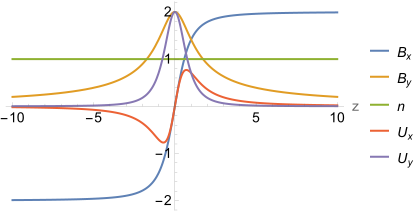
\includegraphics{article_files/mediabag/figures/profiles_sym.pdf}\end{minipage}%
%
\begin{minipage}{0.50\linewidth}
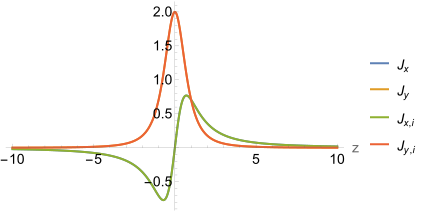
\includegraphics{article_files/mediabag/figures/J_profiles_sym.pdf}\end{minipage}%

\caption{\label{fig-profiles}(a). Magnetic field, ion density, and ion bulk velocity for \(n_1 = n_2, u_1 = -u_2\) and \(δ_1=1, c_1=1/\sqrt{2}, B_0 = 2\). (b). Current density profiles for the same case.}

\end{figure}%

\subsection{Alfvenicity}\label{alfvenicity}

For the same asymptotic magnetic field, it is interesting to see how the plasma profiles change with different system parameters.

Here we set \(B_y(z=\infty) = 1/2 B_0, B_0 = 2 B_z\), and let two ion species have the opposite bulk velocity but this time with different densities. By varying \(n_1(∞)\), we find that the magnetic field profiles are exactly the same, while plasma density and velocity profiles vary.

We normalize the plasma velocity by asympotic Alfvén velocity \(v_{A}(∞) = B_0 / \sqrt{\mu_0 m_i n}\), and the profiles are plotted below Figure~\ref{fig-profilesC}. It could be seen that for \(n_1(∞) = 0.5\), we have zero bulk velocity change across the current sheet in the asymptotic limit. And the change of bulk velocity across the current sheet increases with \(n_1(∞)\) decreasing to zero Figure~\ref{fig-uxnorm}. The normalized plasma velocity \(U_y\) in the aympotic limit decreases with \(n_1(∞)\) decreasing to zero Figure~\ref{fig-uynorm}.

\begin{figure}

\begin{minipage}{0.25\linewidth}

\centering{

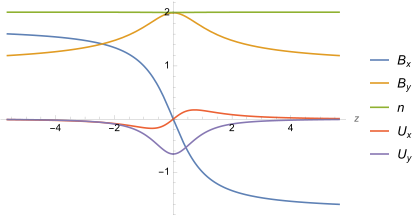
\includegraphics{article_files/mediabag/figures/profiles_ratio=0.5.pdf}

}

\subcaption{\label{fig-profiles_ratio}Magnetic field, ion density, and ion bulk velocity for two ion species with same bulk velocity but different densities.}

\end{minipage}%
%
\begin{minipage}{0.25\linewidth}

\centering{

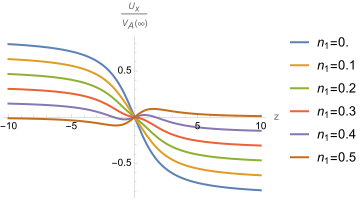
\includegraphics{article_files/mediabag/figures/UxNormB0.pdf}

}

\subcaption{\label{fig-uxnorm}Plasma velocity \(U_x\) profiles normalized by aysmpotic Alfvén velocity for different \(n_1(∞)\).}

\end{minipage}%
%
\begin{minipage}{0.25\linewidth}

\centering{

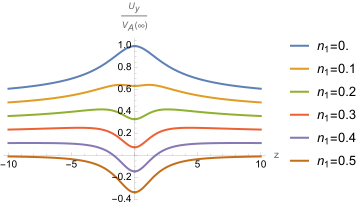
\includegraphics{article_files/mediabag/figures/UyNormB0.pdf}

}

\subcaption{\label{fig-uynorm}Plasma velocity \(U_y\) profiles normalized by aysmpotic Alfvén velocity for different \(n_1(∞)\).}

\end{minipage}%
%
\begin{minipage}{0.25\linewidth}

\end{minipage}%

\end{figure}%

Normalized by Alfvén velocity \(v_{A,x}\) and \(v_{A,y}\), the plasma velocity profiles are plotted below Figure~\ref{fig-uxNormBx} and Figure~\ref{fig-uyNormBy}. The normalized plasma velocity profiles are exactly the same for \(U_x/v_{A,x}\) and \(U_y/v_{A,y}\) for same \(n_1(∞)\). When \(n_1(∞)\) decreases to zero, the normalized plasma velocity would approach one in the asymptotic limit, indicating the Alvenicity of the current sheet.

\begin{figure}

\begin{minipage}{0.50\linewidth}

\centering{

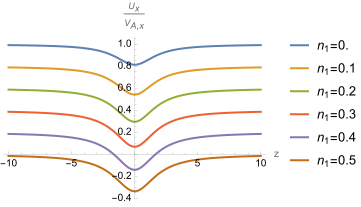
\includegraphics{article_files/mediabag/figures/UxNormBx.pdf}

}

\subcaption{\label{fig-uxNormBx}Plasma velocity \(U_x\) profiles normalized by \(v_{A,x}\) for different \(n_1(∞)\).}

\end{minipage}%
%
\begin{minipage}{0.50\linewidth}

\centering{

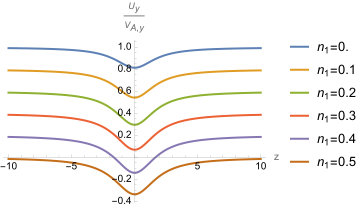
\includegraphics{article_files/mediabag/figures/UyNormBy.pdf}

}

\subcaption{\label{fig-uyNormBy}Plasma velocity \(U_y\) profiles normalized by \(v_{A,y}\) for different \(n_1(∞)\).}

\end{minipage}%

\end{figure}%

The asymptotic velocity for the each species, bulk velocity and normalized one by Alfvén velocity are plotted below Figure~\ref{fig-vRatios} and Figure~\ref{fig-vRatiosEx2} for the case of \(\lambda_{z,2} = - 1\) (two groups of opposite velocity in z direction) and \(\lambda_{z,2} = - 1/2\) respectively. For the case of \(\lambda_{z,2} = - 1\) as shown in Figure~\ref{fig-vRatiosEx1}, the normalized velocity reaches zero when \(n_1(∞) = 0.5\). The bulk velocity of each species is the same in the asymptotic limit and does not depend on \(n_1(∞)\). However, this does not generally hold when \(\lambda_{z,2} \neq - 1\) as shown in Figure~\ref{fig-vRatiosEx2} for the case of \(\lambda_{z,2} = - 1/2\).. The normalized velocity reaches zero when \(n_1(∞) = 1/3\), and the bulk velocity of each species differs in the asymptotic limit and depends on \(n_1(∞)\).

\begin{figure}

\begin{minipage}{0.50\linewidth}

\centering{

\captionsetup{labelsep=none}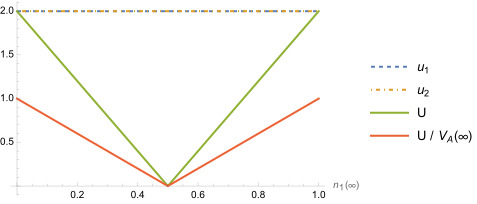
\includegraphics{article_files/mediabag/figures/vRatios.pdf}

}

\subcaption{\label{fig-vRatiosEx1}}

\end{minipage}%
%
\begin{minipage}{0.50\linewidth}

\centering{

\captionsetup{labelsep=none}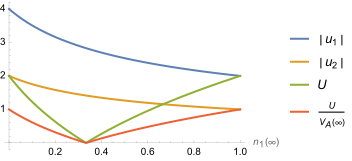
\includegraphics{article_files/mediabag/figures/vRatiosEx2.pdf}

}

\subcaption{\label{fig-vRatiosEx2}}

\end{minipage}%

\caption{\label{fig-vRatios}Asymptotic velocity for each species, bulk velocity and normalized one by Alfvén velocity for the case of \(\lambda_{z,2} = - 1\) (a) and \(\lambda_{z,2} = - 1/2\) (b).}

\end{figure}%

\subsection{Current Sheet Thickness}\label{current-sheet-thickness}

TODO: define and compare current sheet thickness

TODO: compare with Harris current sheet solution with same thickness

\subsection{Density Peaking}\label{density-peaking}

\section{Summary}\label{summary}

\begin{figure}

\centering{

\includegraphics{article_files/mediabag/vl_ratio.png}

}

\caption{\label{fig-vRatioStats}Statistics of the asymptotic velocity ratio from PSP, Wind, and ARTEMIS spacecraft observations during PSP encounter 7 period from 2021-01-14 to 2021-01-21.}

\end{figure}%


  \bibliography{files/bibliography/research.bib}


\end{document}
